\chapter{Games and emotions}
\label{ch:literature-games}

Research about games is a broad topic that involves different disciplines and definitions. In the context of this thesis proposal, a game is defined as a system in which players engage in an artificial conflict, defined by rules, that results in a goal \parencite{salen2004rules}. An artificial conflict is a set of challenges that the player must overcome towards the game goal, e.g. sort elements within a time constraint.

\textcite{schell2014art} mentions that, from a game design perspective, the difficulty level of such challenges affects the emotional state of players, e.g. moments of boredom or anxiety/stress. Every time a reward is given to the player, which usually is a tool to increase the player's power, the game's challenge level is lowered because the player becomes more skilled. After a period, such increase in the player's skill level causes the game to be boring because the challenges are now easier to beat. At that point, the difficulty level is again increased by the game, raising the challenging levels for the player once more, causing anxiety. The anxiety and stress period lasts until the player is rewarded again, when the newly obtained power will eventually lower the challenge levels again (resulting in boredom), causing the cycle to repeat itself.

\textcite{chen2007flow} used the theory of flow or the ``theory of optimal experience'', originally estaslished by \textcite{csikszentmihalyi1991flow}, to describe how player experience was in large part depending on the relationship between a game's challenge and its player's level of skill. A challenge beyond the player's skill to address and overcome it causes anxiety, while the opposite results in disinterest, leading to boredom \parencite{chen2007flow}. An ideal challenge/skill balance in a repeating cycle of increasing challenge followed by a reward keeps the player in an optimal experience and concentration, i.e. flow zone, as illustrated by Figure \ref{fig:flow-schell}.

\begin{figure}[h!]
    \centering
    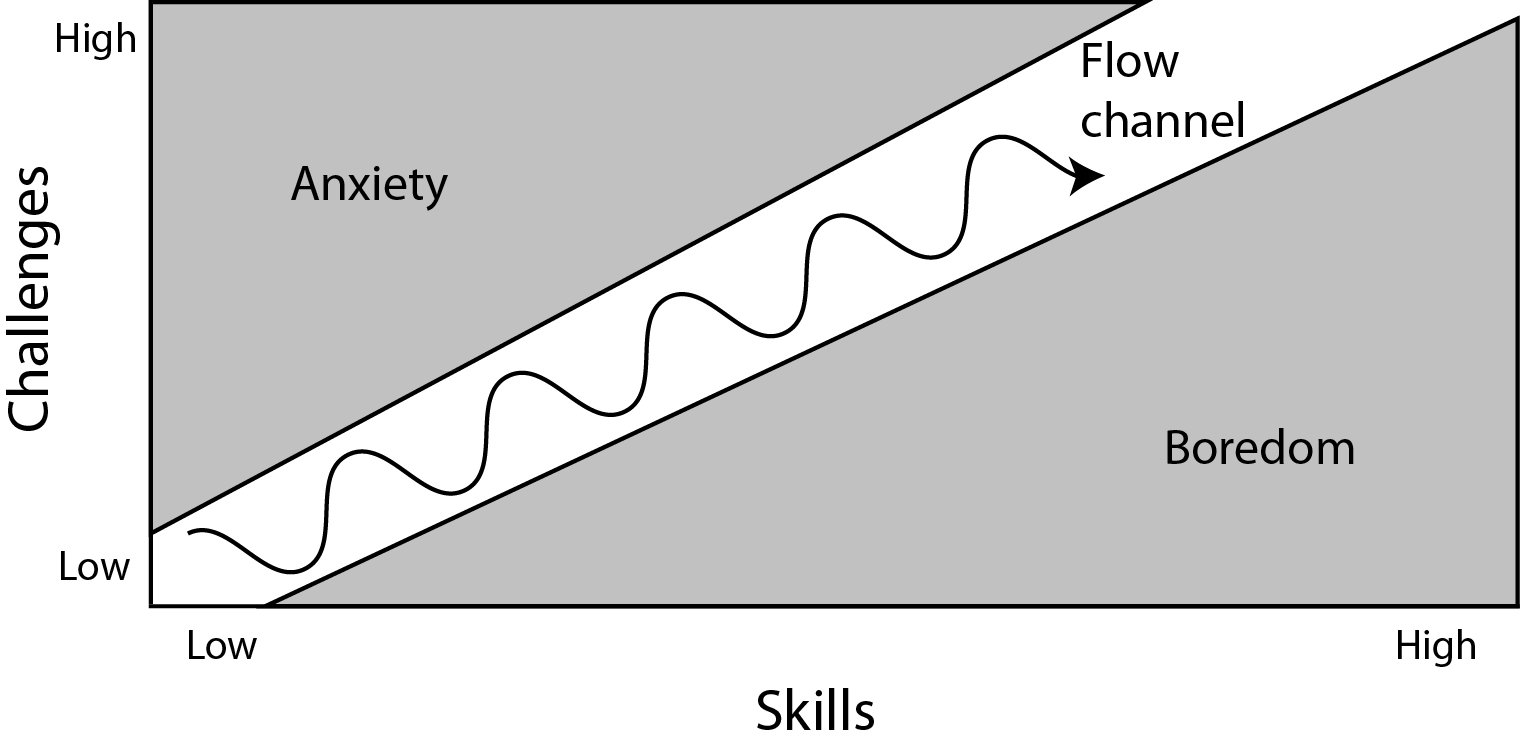
\includegraphics[scale=0.8]{figures/flow-schell.png}
    \caption{Repeating cycle of increasing challenge followed by a reward, keeping the player in the flow zone. \parencite{schell2014art}}
    \label{fig:flow-schell}
\end{figure}

 The following sections describe in more detail the theoretical foundation of emotions, connecting them to the context of games.

%%%%%%%%%%%%%%%%%%%%%%%%%%%%%%%%%%%%%%%%%%%%%%%%%%%%%%%%%%%%%%%%%%%%%%%%%%%%%%%%%%%%%%%%%%%%%%%%%%%%%%%
\section{Emotions theory}
%%%%%%%%%%%%%%%%%%%%%%%%%%%%%%%%%%%%%%%%%%%%%%%%%%%%%%%%%%%%%%%%%%%%%%%%%%%%%%%%%%%%%%%%%%%%%%%%%%%%%%%

In the field of games research, one of the most mentioned theories regarding emotions is the theory of flow. It has been used as the foundation for several concepts, including engagement and immersion \parencite{brown2004grounded}, sense of presence \parencite{weibel2011immersion} and applicability in game design \parencite{sweetser2005gameflow, chen2007flow, cruz2017player}. Flow was originally defined as a phenonmenon in which a person experiences a subjective state characterized by an instense level of attention during the execution of an intrinsically motivated activity \parencite{csikszentmihalyi1991flow}. As previously mentioned, an ideal challenge/skill balance in a game leads players to an optimal experience and concentration state (e.g. flow), so flow constructs are of interest to the games community. Such peculiar state of flow, however, is not limited to activities involving games, it can be experienced in a variety of other activities, e.g. dancing and climbing. The connection of the theory of flow to contexts other than games is outside the scope of this thesis proposal.

Further research \parencite{nakamura2014concept} refined the original definition of the flow state, culminating in the eight channel model of flow, illustrated in Figure \ref{fig:flow-eight}. Such model better describes the emotional state of users according to the challenge/skill balance in relation to the subject mean, since it is less coarse than the original flow model. In the eight channel model of flow, for instance, a person performing a low skill and low challenging task experiences apathy, while in the original model the classification would indicate a flow state. Emotional states as stress and boredom can be described as a function of the current player's skill level and the level of challenge he/she is facing.

\begin{figure}[h!]
    \centering
    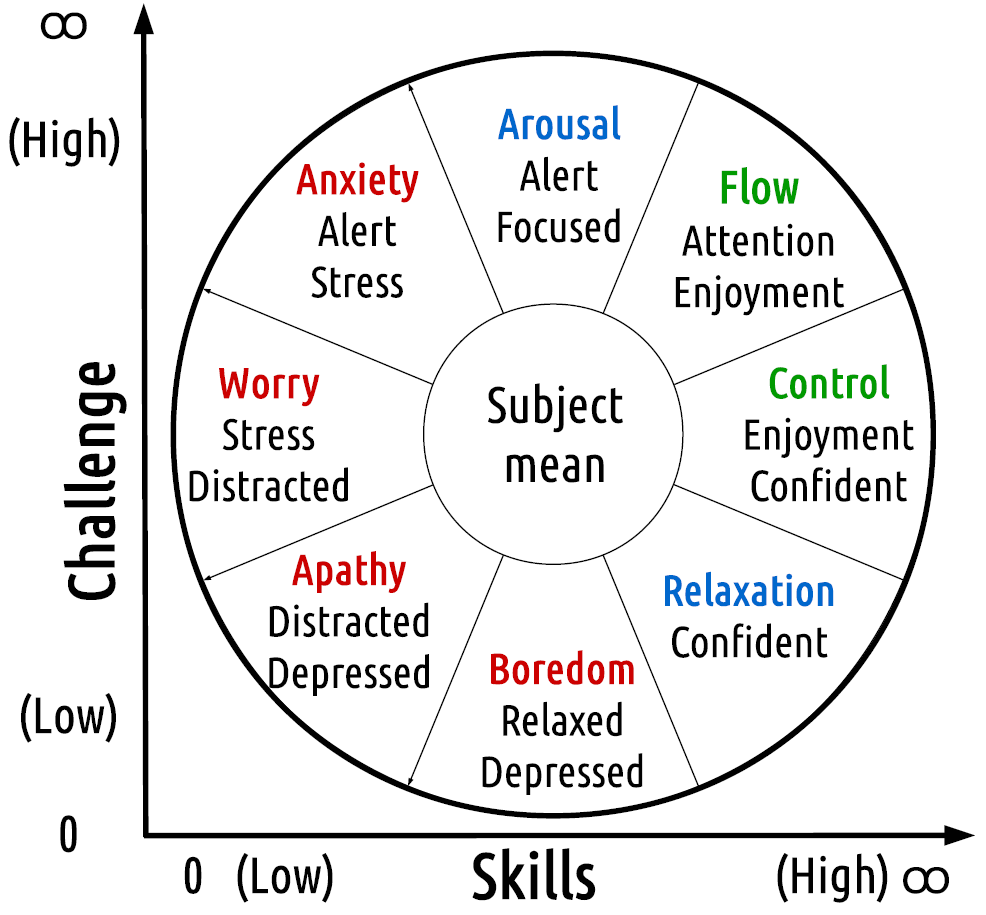
\includegraphics[scale=0.3]{figures/flow-eight.png}
    \caption{Eight channel model of flow \parencite{nakamura2014concept}}
    \label{fig:flow-eight}
\end{figure}

Another model commonly mentioned in the literature are the basic emotions proposed by \textcite{ekman1971constants}. Constructed from an experiment involving cultural differencies, it states that particular facial muscular patterns and discrete emotions are universal. The six emotions mentioned in the theory are happiness, surprise, sadness, fear, anger and disgust, which are strictly basic emotion models of affective state. A contrary definition is presented by \textcite{russell1978evidence}, who defined another model of emotions named Circumplex Model of Affect (CMA). Commonly referred to as Russell's Arousal-Valence (AV) space, the model is contrary to strictly basic emotion models of affective state, where each emotion emerge from independent neural systems \parencite{posner2005circumplex}. The model proposes a dimensional approach where all affective states arise from the activation of two fundamental neurophysiological systems: arousal (or alertness) and valence (a pleasure–displeasure continuum).

\begin{figure}[h!]
    \centering
    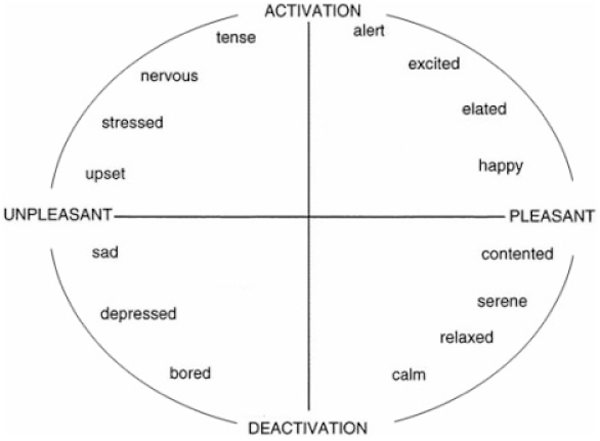
\includegraphics[scale=0.5]{figures/russell-av.png}
    \caption{Representation of the circumplex model of affect \parencite{posner2005circumplex}. Horizontal axis represents the valence dimension and the vertical axis represents the arousal or activation dimension.}
    \label{fig:av-model}
\end{figure}

Figure \ref{fig:av-model} illustrates the AV space. The horizontal axis represents the valence dimension, which varies from the negative, unpleasant spectrum to the positive, pleasant spectrum. The vertical axis represents the arousal or activation dimension, which varies from low (bottom) to high (top). Each emotion is the result of a linear combination of these two dimentions. An emotional state of excitement, for instance, is conceptualized as the product of a positive activation in the neural system associated with valence along with a high activation in the neural system associated with arousal. The different scales of activation of each of those two dimensions produces different emotional states.

%%%%%%%%%%%%%%%%%%%%%%%%%%%%%%%%%%%%%%%%%%%%%%%%%%%%%%%%%%%%%%%%%%%%%%%%%%%%%%%%%%%%%%%%%%%%%%%%%%%%%%%
%\section{Stress, boredom and flow}
%%%%%%%%%%%%%%%%%%%%%%%%%%%%%%%%%%%%%%%%%%%%%%%%%%%%%%%%%%%%%%%%%%%%%%%%%%%%%%%%%%%%%%%%%%%%%%%%%%%%%%%

%%%%%%%%%%%%%%%%%%%%%%%%%%%%%%%%%%%%%%%%%%%%%%%%%%%%%%%%%%%%%%%%%%%%%%%%%%%%%%%%%%%%%%%%%%%%%%%%%%%%%%%
\section{Immersion, engagement and sense of presence}
%%%%%%%%%%%%%%%%%%%%%%%%%%%%%%%%%%%%%%%%%%%%%%%%%%%%%%%%%%%%%%%%%%%%%%%%%%%%%%%%%%%%%%%%%%%%%%%%%%%%%%%

As previously mentioned, the theory of flow is significantly used to explain emotional states and concepts in the field of games research. The definition of flow, however, requires a more sophisticated interpretation, as investigated by further research. %As previously mentioned, from a game design perspective, for instance, Schell \parencite{schell2014art} mentions that a progression of the player in the flow zone is desired, however it should not be a ``straight line'', but more of a cycle alternating among emotional states as stress, enjoyment and boredom.
Different elements are also connected to flow, such as engagement, immersion and sense of presence.

Immersion, in the concept defined by \textcite{brown2004grounded}, refers to the degree of involvement of players with a computer game. In that light, the authors theorize that a player overcomes barriers that limit his/her degree of involvement in immersion. After each barrier is broken, the sense of immersion deepens. The first barrier, for instance, is named engagement and it refers to the player willingness to invest attention and energy to learn how to play the game. The concept of flow, as defined by \textcite{csikszentmihalyi1991flow}, is an extreme state, which is only achieved when the player has overcame all previously mentioned barriers and is in a ``total immersion'' state. Such condition is rare to happen since it requires the highest level of attention from the player. As a consequence, engagement is more plausible and common during gaming experiences than flow.

The existence of several works \parencite{boyle2012engagement} related to understanding and defining what engagement and immersion are demonstrates the interest of researchers to broaden the view beyond flow alone. Presence, for instance, which describes the player's feeling of actually being in the game, is reported as an important aspect of engagement and immersion \parencite{weibel2011immersion}. Studies connected to training simulation \parencite{engstrom2016impact}, for instance, also indicate that contextualization (increasing the sense of presence) might affect immersion positively. Additionally to the intentions of understanding and defining engagement and immersion, studies also try to measure them. The majority of the approaches used for that are based on questionnaires, which are by nature subjectively answered by players. Additionally that approach usually breaks any sense of presence of the player since it requires a shift in attention away from the game, hence breaking or affecting the level of engagement/immersion as well.

Quantitative approaches have also been investigated to measure engagement, such as the use of physiological signals like heart rate \parencite{ravaja20051} and eye movement \parencite{jennett2008measuring}, for instance. The complexity in defining engagement and immersion is also reflected in the task of measuring it. \textcite{ravaja20051}, for instance, mentions the significant variation of physiological signals as an obstacle. Signals increase during emotional arousal, but decrease in response to attention engagement, which makes the measurement of engagement a non-trivial process. It highlights the difficulties in correlating qualitative data to more abstract concepts as engagement, immersion and flow.

%Research initiatives that help in the identification of the player emotional state without breaking the current level of engagement and immersion are desired. This research aims at using the link between the ANS and emotional regulation as the foundation to analyse physiological signals of a player, which will be remotely obtained and processed in a user-tailored fashion according to data previously collected in a game-based calibration phase.
